\section{Related Work}
The goal of this project was to create a new kickable and flickable interface for outdoors. For this, we first did some research about interactive systems that were designed for public spaces and interfaces that focused on feet interaction. Here, we present some interesting systems that inspired us during the creative phase of our work.
 
Seitinger, S. et al. \cite{seitinger} created the 'Light bodies'(see Figure~\ref{fig:Light bodies}): mobile and portable, hand-held lights that respond to audio and vibration input. Street lighting has changed over time and its relation to individuals has been also altered as a result. In the middle ages, each person used its own lantern. Then, in the beginning of 18th century, cities like Paris started to illuminate their streets at night; personal lanterns were not longer required. 'Light bodies' is an attempt to bring back the lost connection between lanterns and people and a medium to investigate the relationships between (urban) spaces, light and responsive, hand-held lights.'Light bodies' enabled people to directly and indirectly influence their personal lightscape.

\begin{figure}[h!]
	\centering
	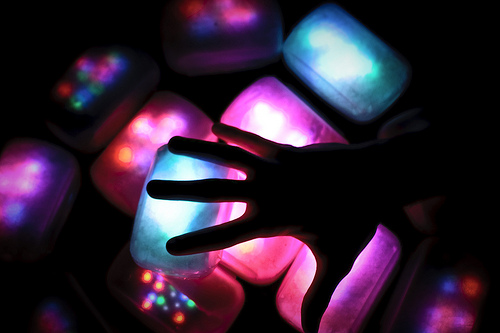
\includegraphics[width=0.45\textwidth, clip=true, keepaspectratio=true]{./pic/light-bodies.jpg}
	\caption{Light bodies}
	\label{fig:Light bodies}
\end{figure}


In another related project, Seitinger, S. et al. \cite{seitinger-2} designed and implemented the 'Urban pixels': physically instantiated pixels that enable flexible, reconfigurable, unbounded, low-resolution, and responsive urban displays (see Figure~\ref{fig:urban-pixels}). 'Urban Pixels' are nodes in a wireless network of physical pixels for urban spaces. Each pixel unit includes a microcontroller, RF transceiver, LED module (ten bright, white LEDs), rechargeable Li-Ion battery pack, IR sensor and renewable energy source such as photo-voltaic cells. Users can interact with the 'urban pixels' by placing them spontaneously, by triggering sensors or by sending messages from their mobile devices. 

\begin{figure}[h!]
	\centering
	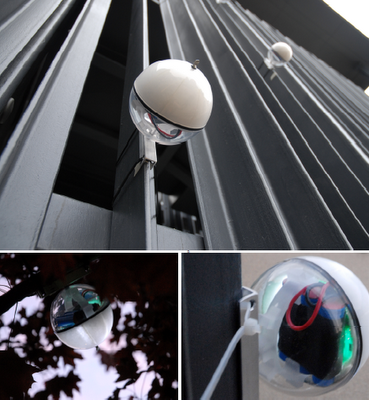
\includegraphics[width=0.2\textwidth, clip=true, keepaspectratio=true]{./pic/urban-pixels.png}
	\caption{Urban-pixels}
	\label{fig:urban-pixels}
\end{figure}

With this design, Seitinger, S. et al. \cite{seitinger-2} wants to present an opposite alternative to the majority of displays that are inflexible, flat, bounded, high-resolution and unresponsive. 

As an example of an interface where feet play the main role, Paelke et al. \cite{paelke} implemented a system for foot-based mobile interaction, which uses a camera of current video capable mobile devices to detect motion and position of the user’s foot to effect the input
that is required for simple games like \emph{Pong}, \emph{Break-out} or \emph{soccer}. Figure~\ref{fig:feet-based-game} shows an scenario where a user interacts with its mobile phone by moving one feet. 

\begin{figure}[h!]
	\centering
	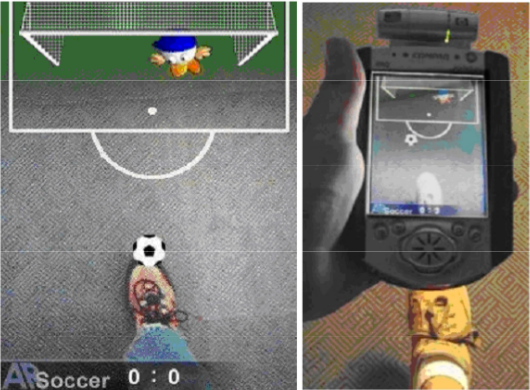
\includegraphics[width=0.25\textwidth, clip=true, keepaspectratio=true]{./pic/foot-based-game.png}
	\caption{Mobile phone game and user interacting with it by moving a foot}
	\label{fig:feet-based-game}
\end{figure}
